%-----------------------------------------------------------------------------------%
\section{The Detector}
%-----------------------------------------------------------------------------------%

\begin{figure}[h!]
    \centering{
    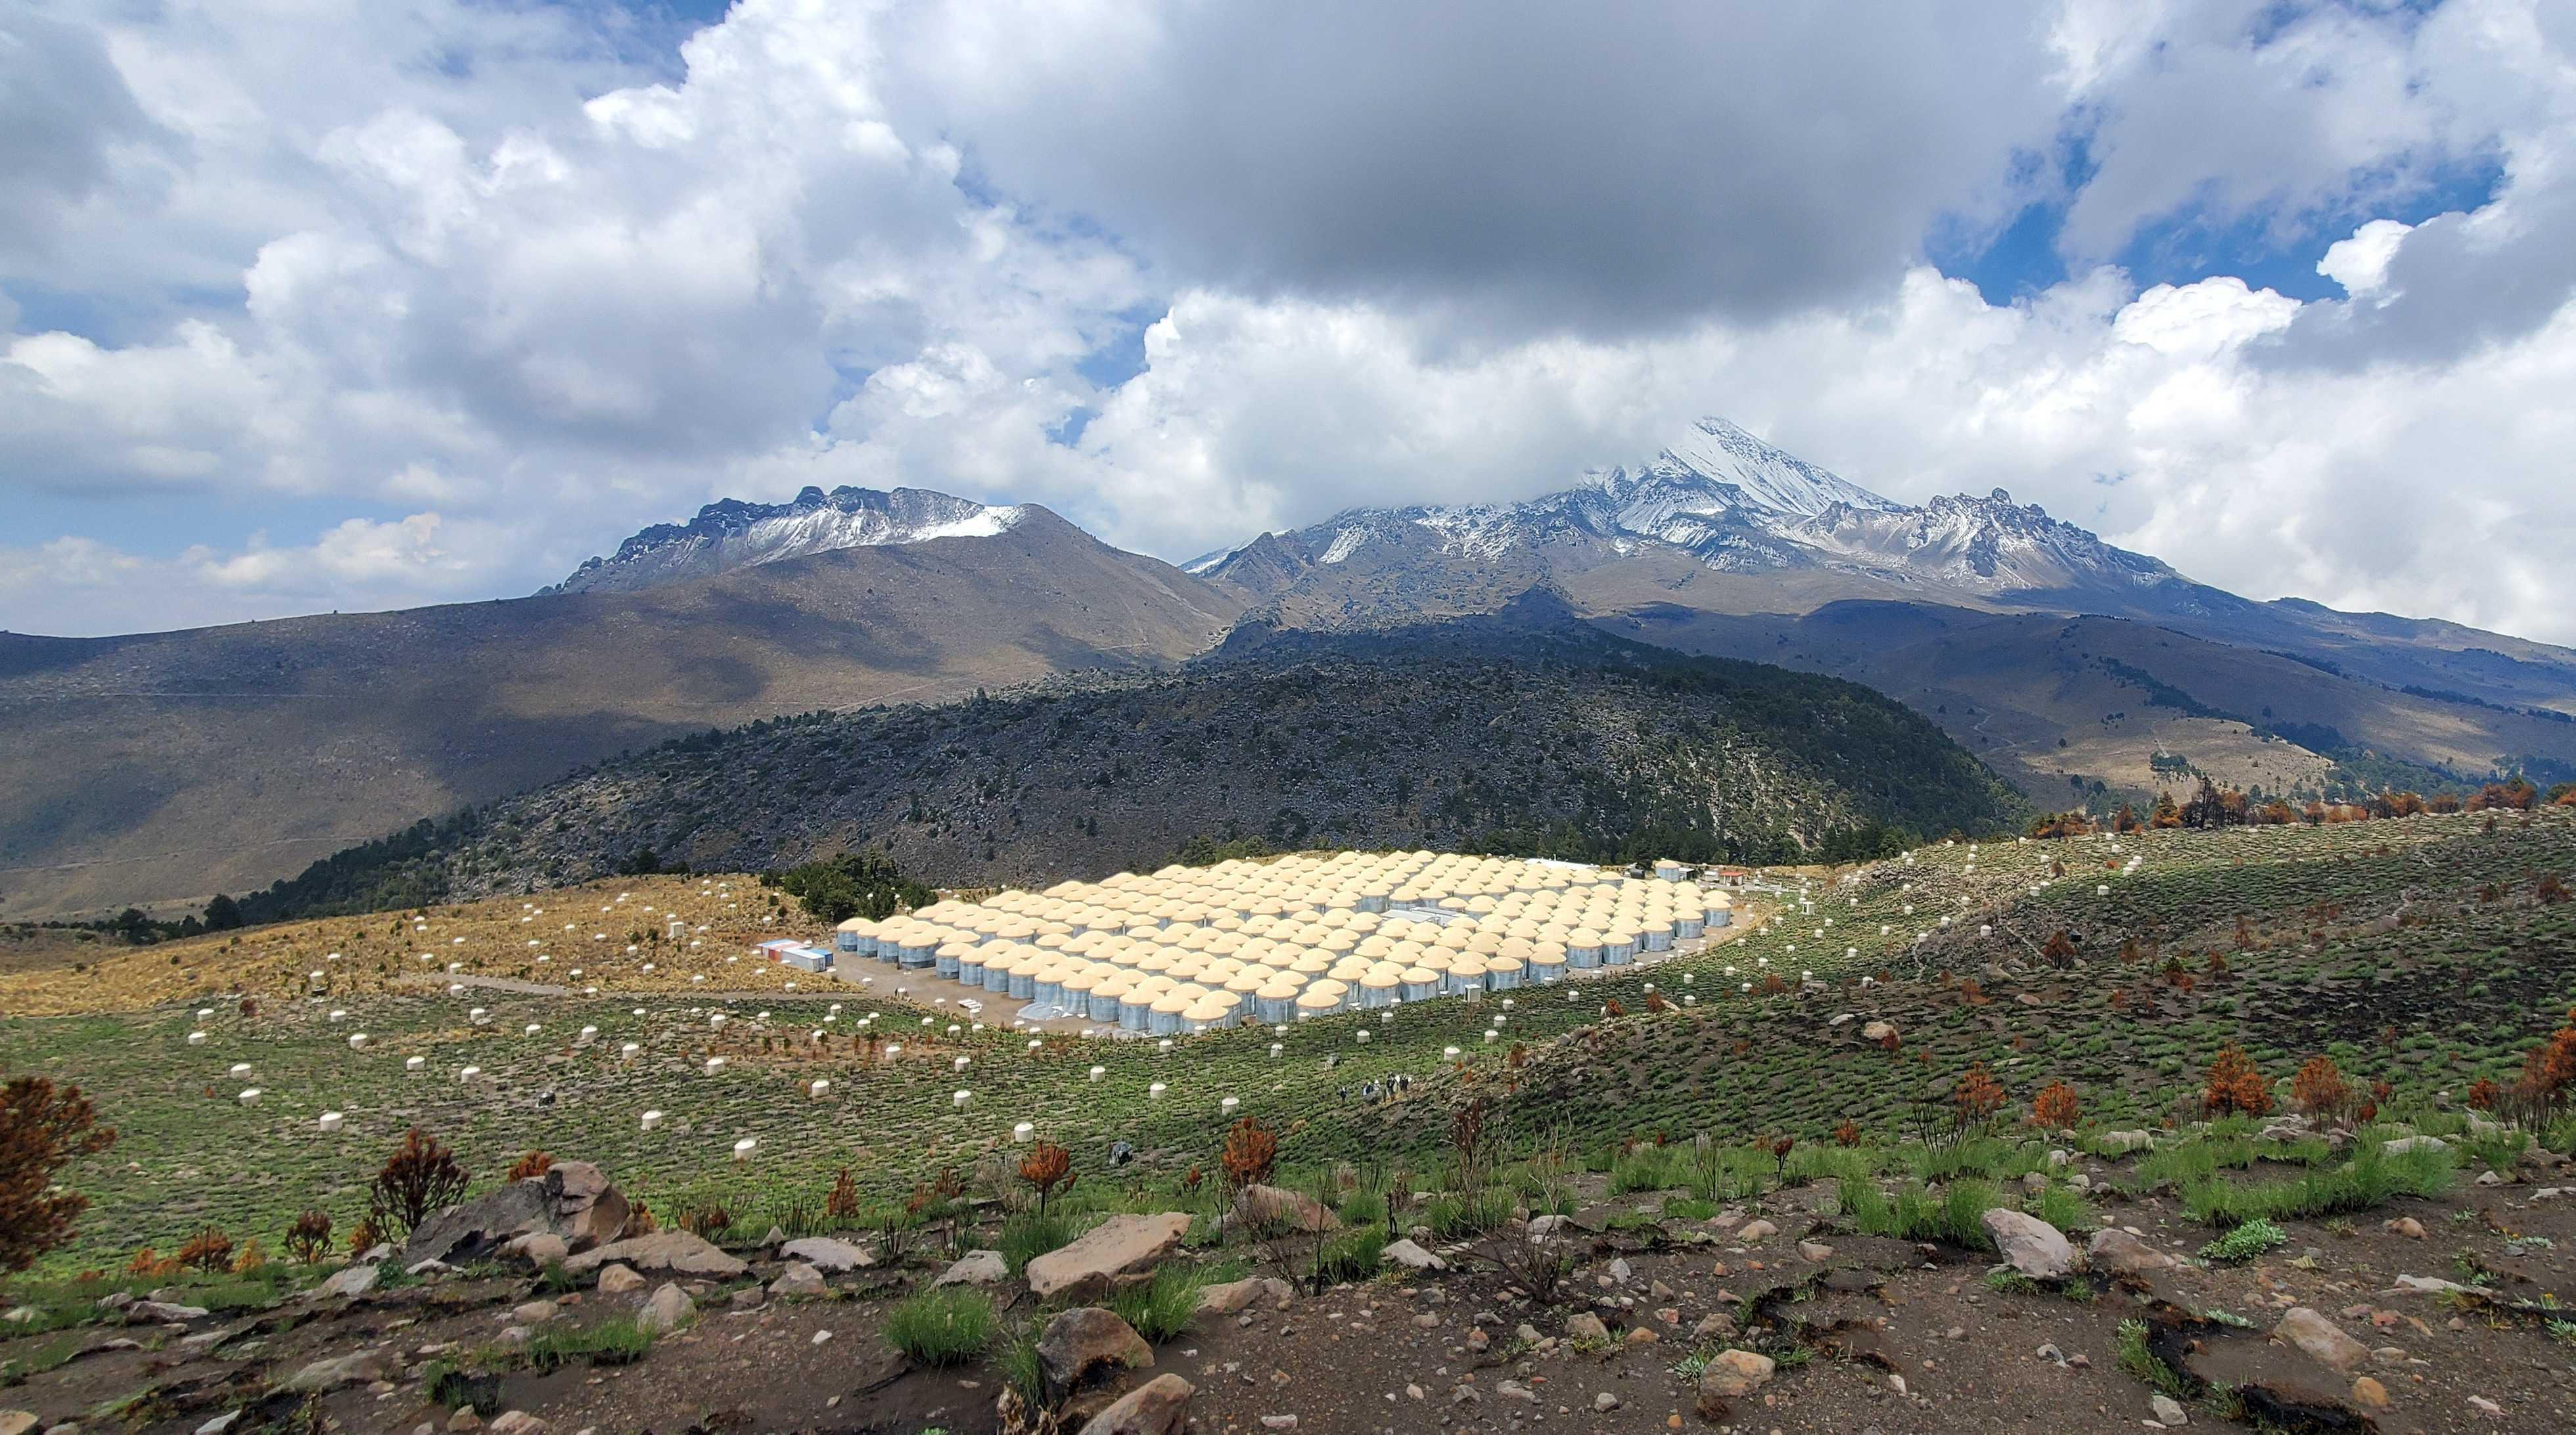
\includegraphics[scale=0.155]{figures/hawc/HAWC.jpg}
    }
    \caption{Photo of the HAWC detector that I took on May 17, 2023. Main array is centered in the photo and comprised of the larger tanks. Outriggers are the smaller tanks around the main array.}
    \label{fig:HAWC}
\end{figure}

The High Altitude Water Cherenkov (HAWC) Observatory is a specialized instrument designed for the observation of high energy gamma-rays and cosmic rays \cite{HAWC_NIM}.
Located on the Sierra Negra volcano in Mexico, HAWC observes gamma rays and cosmic rays in the energy range of approximately 100 GeV to 100'ss of TeV.
HAWC is strategically situated to maximize observational efficiency due to its high altitude.
At an elevation of 4,100 meters, it monitors about two-thirds of the sky every day with an uptime above 90\%.
This capability is essential for studying high-energy astronomical phenomena.

HAWC comprises of 300 water Cherenkov detectors (WCDs) spread over 22,000 square meters.
Each main array detector is filled with purified water and equipped with four, upward-facing photomultiplier tubes (PMTs).
These PMTs detect Cherenkov radiation from charged particles passing through the tanks.
These charged particles are generated when a high energy gamma or cosmic ray collides with gas in the atmosphere to create a charged particle shower, see \cref{fig:airshowers}.
The observatory includes a separate tank configuration which are refered to as the outriggers.
They are a secondary array of 345 smaller WCD's.
Surrounding the main array, each outrigger tank measures 1.55 meters in diameter and height and contain a single upward-facing eight-inch PMT.
This expansion increases the instrumented footprint fourfold.
It improves the reconstruction of showers extending beyond the main array, especially for events above 10 TeV.
However, at the time of writing this thesis, the outriggers have not been fully integrated into HAWC's reconstruction software.

\begin{figure}
    \centering{
    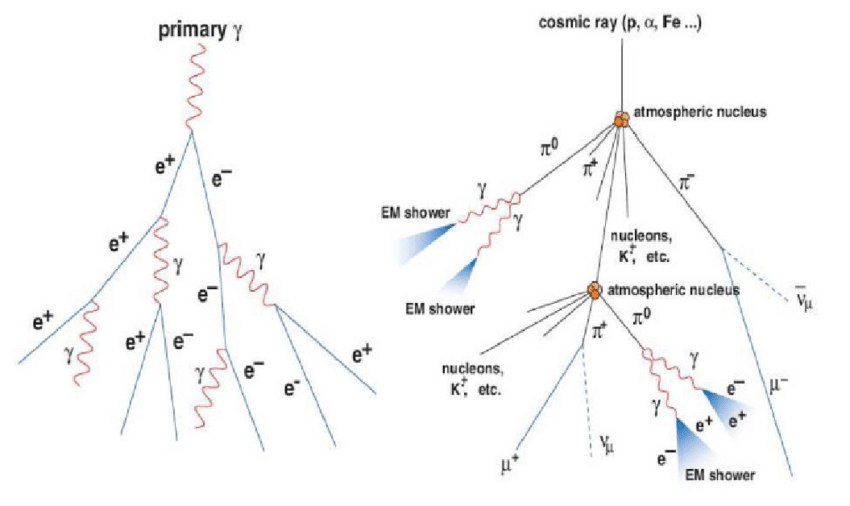
\includegraphics[scale=0.5]{figures/hawc/high_energy_air_shower.png}
    }
    \caption{A particle physics illustration of high energy particle showers. Left shower is an electromagnetic shower from a high energy gamma-ray. Most particles in the shower will be a combination of photons and charged leptons, in this case electrons (e). Right figure shows a cosmic ray particle shower. The cosmic ray will produce many more types of particles including pions ($\pi$), neutrinos, and charged leptons. Figured pulled from \cite{lopez_thesis}.}
    \label{fig:airshowers}
\end{figure}

%-----------------------------------------------------------------------------------%
\section{Construction and Hardware}
%-----------------------------------------------------------------------------------%

\begin{figure}
    \centering{
        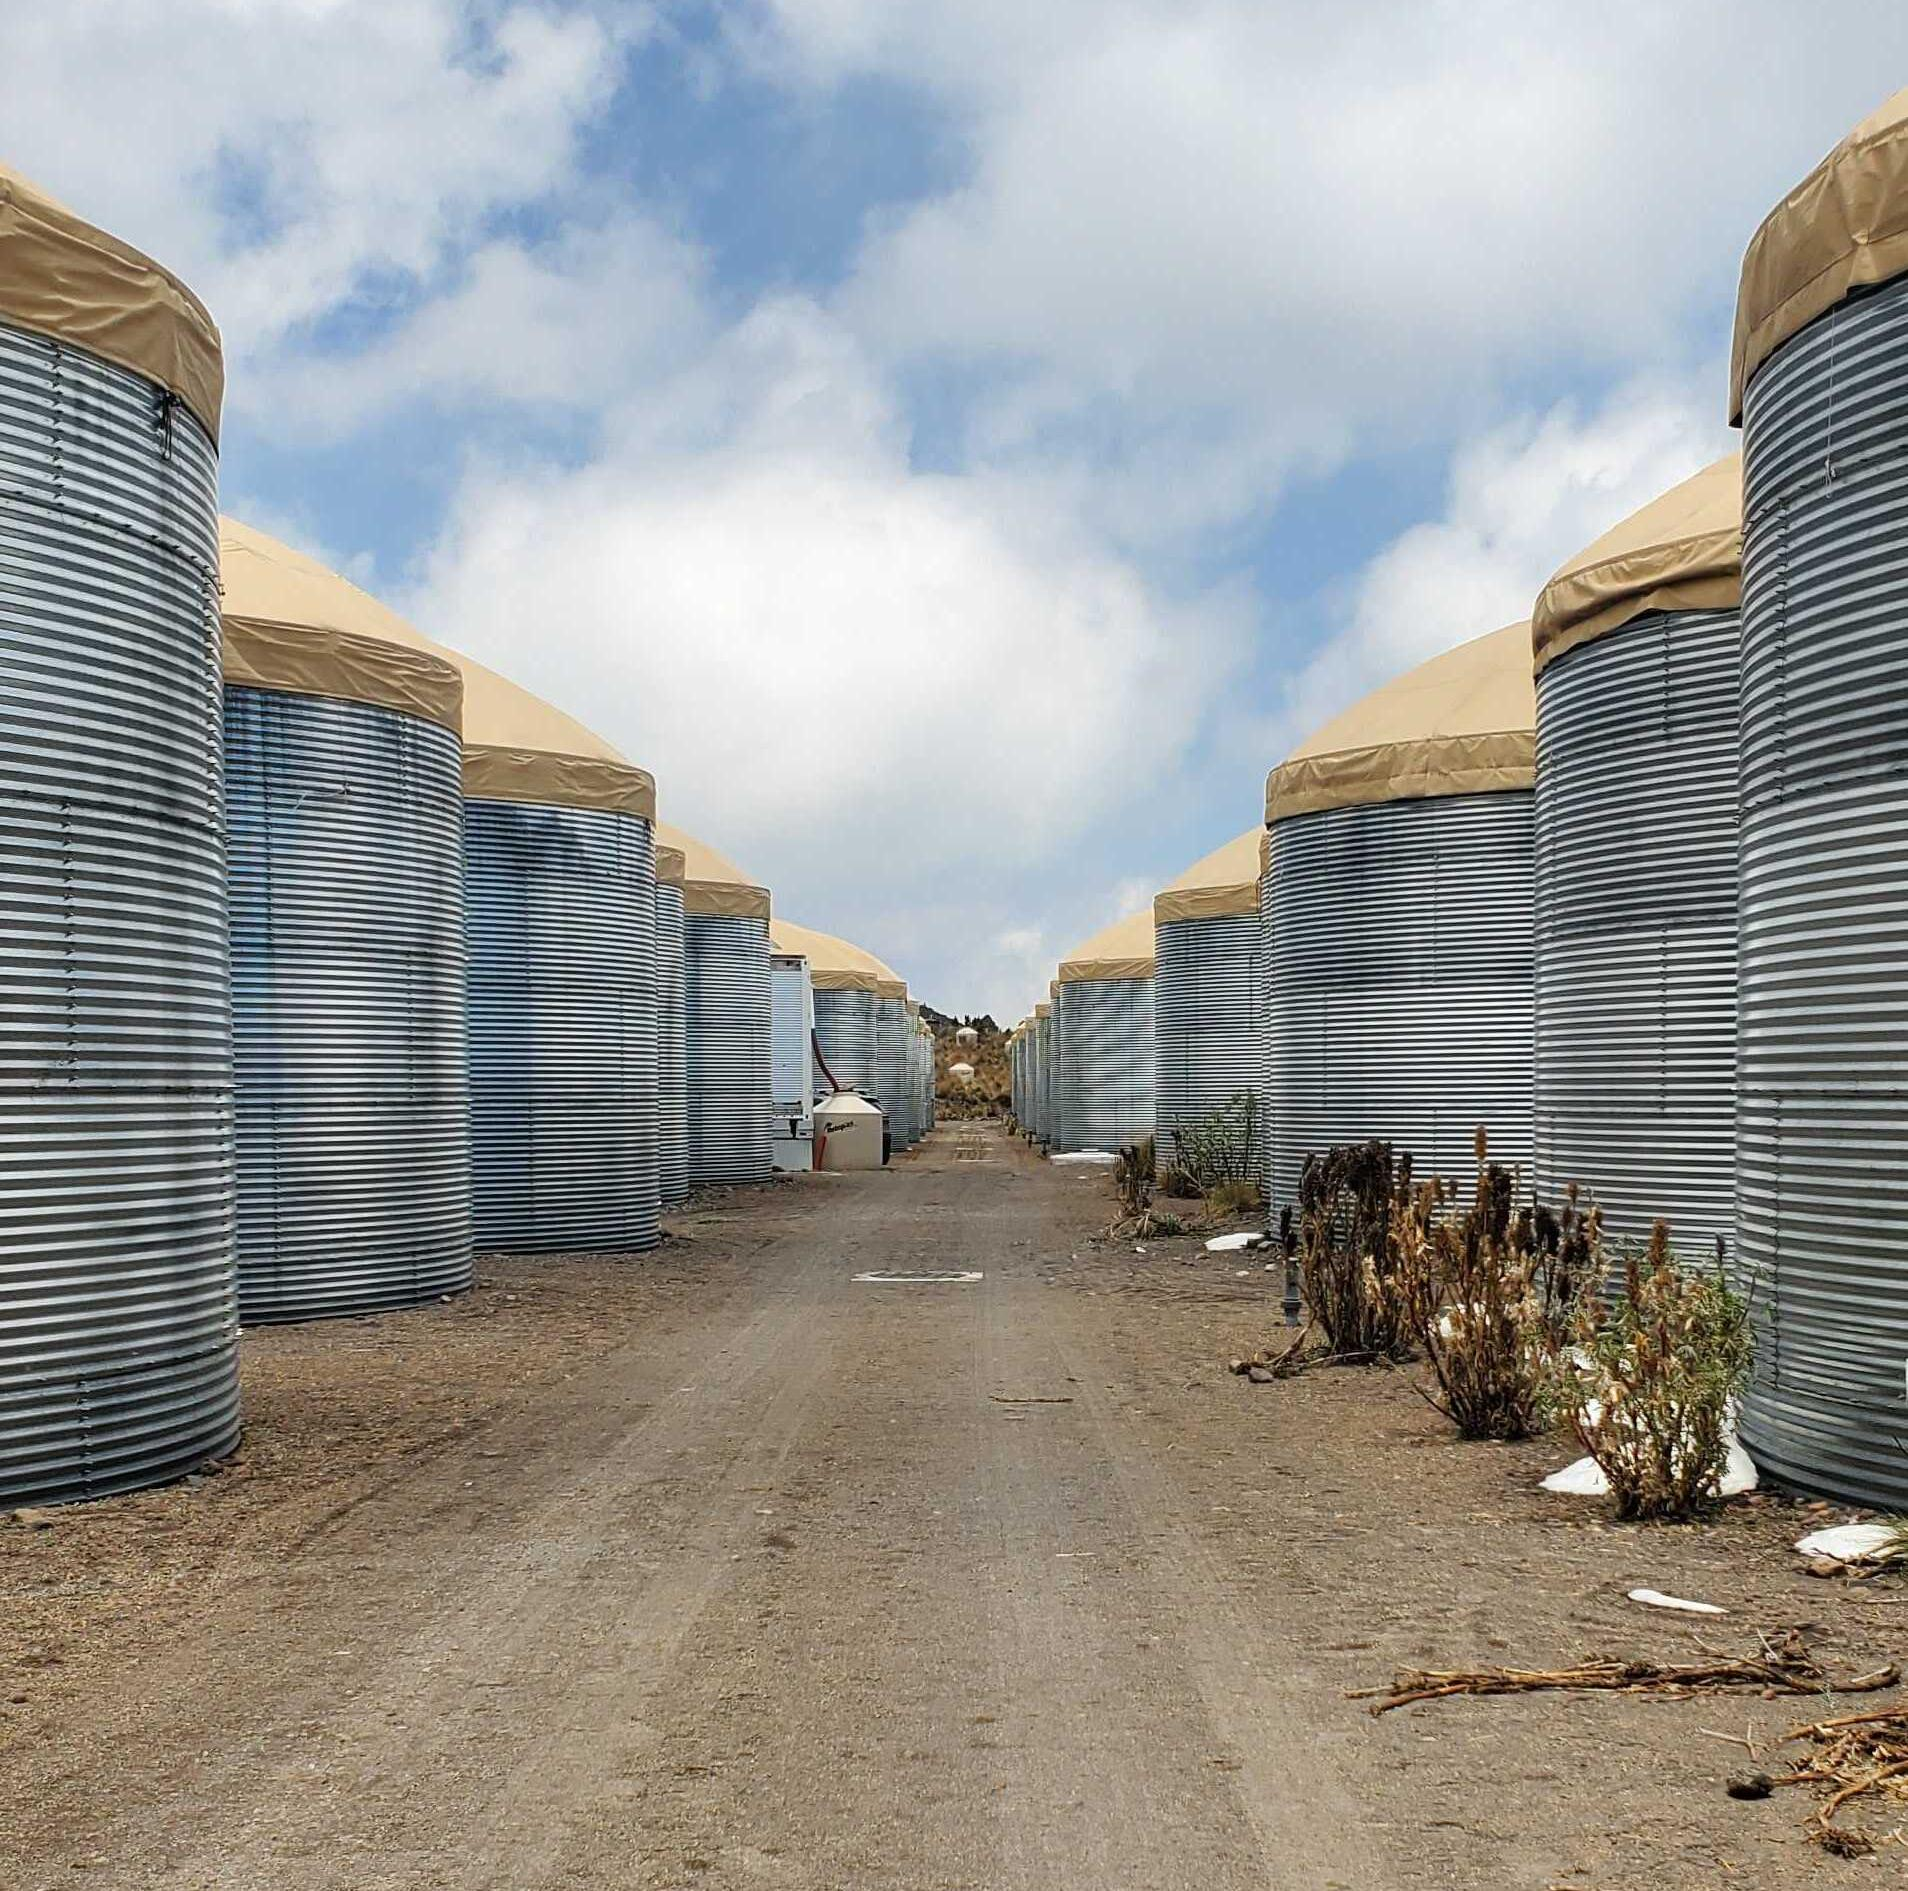
\includegraphics[scale=0.14]{figures/hawc/WCDs.jpg}
        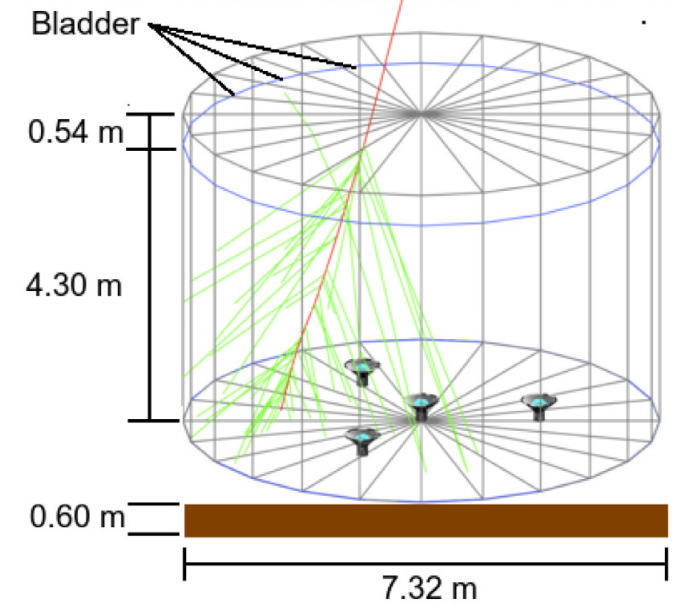
\includegraphics[scale=0.45]{figures/hawc/WCD_schematic.png}
    }
    \caption{The WCDs. Left image features several WCDs looking from within the main array of HAWC. Right image shows a schematic of a WCD pulled from \cite{HAWC_NIM}.}
    \label{fig:WCD_schematic}
\end{figure}
\todo{fact check the content below. GPT may have hallucinated}
Each main array WCD is a cylindrical tank with dimensions of 7.3 m in diameter and 5 m in height \cite{HAWC_NIM}.
The metal shell of these tanks is made from bolted together, corrugated, galvanized steel panels.
This assembly process involves constructing the top ring of panels at ground level, subsequently raising it to add additional rings below until the structure is complete.
The finished tank is placed into a 0.6 m deep trench filled with rammed earth to secure it against seismic activity.
The interior of each tank is lined with a black, low-density polyethylene bladder, designed to be impermeable to external light and to prevent reflection of Cherenkov light within the tank.
This bladder is approximately 0.4 mm thick, composed of two layers of three-substrate film bonded during a co-extrusion process.
To further minimize light penetration, a black agricultural foil covers the bladder, and the ground and walls inside the tank are protected with geo-textile felt and a layer of sand to safeguard against punctures.
The tanks are filled 4.5 m deep of purified water, achieving a photon attenuation length for Cherenkov photons that exceeds the tank's dimensions.
This purification level ensures the optimal detection environment for the photons generated by traversing charged particles.

%-----------------------------------------------------------------------------------%
\section{Events Reconstruction and Data Acquisition}
%-----------------------------------------------------------------------------------%
%$$$$$$$$$$$$$$$$$$$$$$$$$$$$$$$$$$$$$$$$$$$$$$$$$$$$$$$$$$$$$$$$$$$$$$$$$$$$$$$$$$$%
\subsection{G/H Discrimination}
%$$$$$$$$$$$$$$$$$$$$$$$$$$$$$$$$$$$$$$$$$$$$$$$$$$$$$$$$$$$$$$$$$$$$$$$$$$$$$$$$$$$%

%$$$$$$$$$$$$$$$$$$$$$$$$$$$$$$$$$$$$$$$$$$$$$$$$$$$$$$$$$$$$$$$$$$$$$$$$$$$$$$$$$$$%
\subsection{Angle}
%$$$$$$$$$$$$$$$$$$$$$$$$$$$$$$$$$$$$$$$$$$$$$$$$$$$$$$$$$$$$$$$$$$$$$$$$$$$$$$$$$$$%

%$$$$$$$$$$$$$$$$$$$$$$$$$$$$$$$$$$$$$$$$$$$$$$$$$$$$$$$$$$$$$$$$$$$$$$$$$$$$$$$$$$$%
\subsection{Energy}
%$$$$$$$$$$$$$$$$$$$$$$$$$$$$$$$$$$$$$$$$$$$$$$$$$$$$$$$$$$$$$$$$$$$$$$$$$$$$$$$$$$$%

%-----------------------------------------------------------------------------------%
\section{Remote Monitoring}
%-----------------------------------------------------------------------------------%

%$$$$$$$$$$$$$$$$$$$$$$$$$$$$$$$$$$$$$$$$$$$$$$$$$$$$$$$$$$$$$$$$$$$$$$$$$$$$$$$$$$$%
\subsection{ATHENA Database}
%$$$$$$$$$$$$$$$$$$$$$$$$$$$$$$$$$$$$$$$$$$$$$$$$$$$$$$$$$$$$$$$$$$$$$$$$$$$$$$$$$$$%

%$$$$$$$$$$$$$$$$$$$$$$$$$$$$$$$$$$$$$$$$$$$$$$$$$$$$$$$$$$$$$$$$$$$$$$$$$$$$$$$$$$$%
\subsection{HOMER}
%$$$$$$$$$$$$$$$$$$$$$$$$$$$$$$$$$$$$$$$$$$$$$$$$$$$$$$$$$$$$$$$$$$$$$$$$$$$$$$$$$$$%
